\section{État de l'art}

\subsection{Vision, Reconstruction 3D}

\subsubsection{Vision classique}

Nos robots seront équipés de caméras de types différents, On va donc commencer par traiter au cas par cas les algorithmes nécessaires pour les caméras.
La caméra la plus courante est la caméra perspective (ou \textit{pinhole} en anglais).
De très nombreux ouvrages existent sur la reconstruction à l'aide d'une caméra perspective, on retrouve notamment  \citetitle{Hartley03Book} de \citeauthor{Hartley03Book} \cite{Hartley03Book}.

A partir d'images successives issues d'un même capteur, nous pouvons reconstruire un modèle 3D de l'environnement parcouru par un humain ou un robot mobile.
La reconstruction se fait sous la forme d'un nuage de points plus ou moins compact en fonction des détails présents dans les images.
Une fois un nuage de points obtenu, nous pouvons affiner ce modèle en effectuant un ajustement de faisceaux (\textit{bundle adjustement}), cette opération consiste à passer un Levenberg-Marquardt\footnote{Algorithme interpolant l'algorithme de Gauss-Newton et l'algorithme de la descente de gradient} sur les données afin de minimiser les erreurs de projection.

On retrouve également les techniques de reconstruction avec deux caméras dans le livre \cite{HoraudBook}, \citetitle{HoraudBook} de \citeauthor{HoraudBook}.

\warning{Cependant une dérive apparaît ...}


\subsubsection{Vision mixte}

L'utilisation complémentaire de caméras omnidirectionnelles, nous pouvons nous demander si nous pouvons utiliser les deux types de caméras simultanément afin de créer le nuage de point.
On retrouve ce genre de travaux quand les travaux de
\citeauthor{Sturm02}, \citetitle{Sturm02} \cite{Sturm02}.
Certains problèmes restent cependant à éclaircir, comme la calibration des caméras omnidirectionnelles.

En lisant ce papier, on se demande alors comment extraire les variables intéressantes comme la matrice essentielle ou les matrices de rotation et de translation.

Une autre question consiste à trouvé un moyen de trouver des points correspondants entre les images perspectives et les images omnidirectionnelles.
Le papier \cite{Puig08} utilise les descripteurs SIFT\footnote{Scale Invariant Feature Transform}.
Il construit ensuite une matrice fondamentale à l'aide des correspondances.
On retrouve des matrices $\mathbf{F}_{43}$, $\mathbf{F}_{63}$ and $\mathbf{F}_{66}$.
On retrouve le même problème que pour le papier précédent pour avoir les matrices importantes \textbf{R} et \textbf{t} ou \textbf{E} depuis $\mathbf{F}_{xx}$?

\newpage

\begin{minipage}[c]{0.5\textwidth}
  \centering
  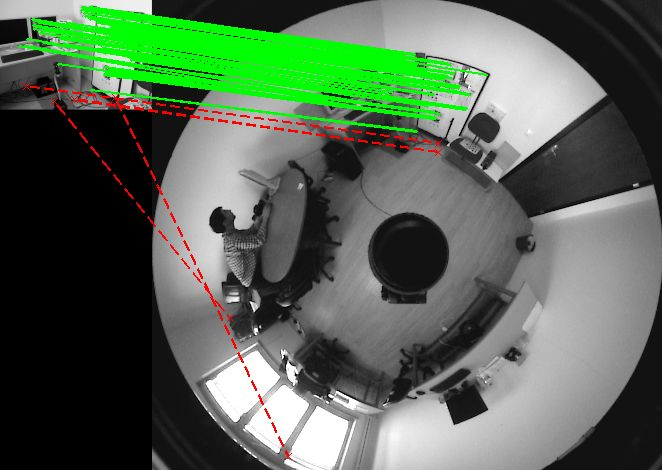
\includegraphics[width=3.0in]{images/Bastanlar09.png}
  \captionof{figure}{Caption for image}
  \label{fig:sample_figure}
\end{minipage}
\begin{minipage}[c]{0.5\textwidth}


  %\begin{tabular}{l l}
  %\begin{minipage}{0.5\linewidth} 
  %\smallfig{0.5}{images/Bastanlar09.png}{[Bastanlar09PhD] Structure from Motion for Systems with Perspective and Omnidirectional Cameras}{fig:bastanlar}
  %\end{minipage}  
  %&
  %\begin{minipage}{0.5\linewidth}
  SfM with hybrid system [Bastanlar09PhD] Structure from Motion for Systems with Perspective and Omnidirectional Cameras\\
  Compute 3D reconstruction with hybrid pair of cameras.\\
  $$q_p^t K_p^{-t} ~E~ \theta^t \hat{K}_c^t \hat{q}_c = 0$$\\
  $\Rightarrow$ No information on calibration of omnidirectional camera $\hat{K}_c$ (see Puig PhD page 25)
  %No information on \textbf{E} computation and \textbf{R},\textbf{t} extraction.
\end{minipage}
%\end{tabular}

%\begin{tabular}{l l}
\smallfig{0.5}{images/Goedeme07.png}{[Goedemé07] Omnidirectional Vision based Topological Navigation}{fig:goedeme}
%&
%\begin{minipage}{0.5\linewidth}

Lorsqu'on a une image, classique ou omnidirectionnelle, nous pouvons nous demander ce que nous devons voir sur cette image.
Quelles sont les amères intéressantes, et pourquoi ?

On retrouve généralement :
\begin{itemize}
\item Le point
\item La droite
\item La courbe
\item L'ellipse ou cercle
\end{itemize}
Chaque type d'amère possède des avantages et des inconvénients :
\begin{table}[h]
  \begin{center}
    \begin{tabular}{|c|c|c|}
      \hline
      Type & Avantages & Inconvénients \\
      \hline
      Point & Générique & Comparaison \\
      Droite & Robuste & Peu présent en extérieur \\
      Courbe & Plus de liberté & Sensible aux rotations \\
      Ellipse & Facile à sélectionner & Peu présent en général\\
      \hline
    \end{tabular}    		
  \end{center}
  \caption{Comparaison des amères}
\end{table}

Nous ne pourrons donc pas utiliser les courbes et les ellipses car pour l'un il nous sera difficile de les définir, et pour l'autre on ne les retrouve pas en assez grand nombre dans un environnement classique.
Les lignes sont particulièrement présentes dans les environnements intérieurs, mais malheureusement beaucoup moins en extérieur.
Notre robots devant naviguer principalement en extérieur, ce type d'amère est incompatible avec notre besoin.
Il reste donc les points, qui sont naturellement présent dans toutes les images nettes d'un environnement.
Le défi sera donc de caractériser les différents points de l'image afin de pouvoir les comparer et les appairer.
Plusieurs outils sont à notre disposition, il s'agit de descripteurs.
On va caractériser une imagette d'une taille fixe autour du point, puis enregistrer l'information en même temps que la position du point dans l'image.

%\end{minipage}
%\end{tabular}
\warning{Répétition}

Dans le cas des images omnidirectionnelles, compte tenu de la déformation des images, les seules amères pouvant être utilisées sont :
\begin{itemize}
\item Les points : les appariements se font avec principalement SIFT
\item Les droites : détection de droites verticales (droites se coupant au centre de l'image), droites parallèles (sous forme de coniques dans l'image)
\end{itemize}



\smallfig{0.2}{images/Dame10.png}{[Dame10PhD] A unified direct approach for visual servoing and visual tracking using mutual information}{fig:dame}
Dame \cite{Dame10PhD} propose un moyen de comparaison de deux imagettes plus performant que les algorithmes proposés : SSD\footnote{Sum of Squared Differences} or ZNCC\footnote{Zero-mean Normalized\\Cross Correlation}.
Comparer MI avec SIFT, SURF et autres descripteurs lors des cas de vision hybride perspective/catadioptrique.  

\subsubsection{Trajectoire}

En reconstruisant le modèle 3D de l’environnement, on obtient également le chemin parcouru lors de la prise des images.
Ce résultat est moins précis qu'avec un GPS car la fréquence d'acquisition des images est généralement plus élevée.

\smallfig{0.2}{images/Rituerto10.png} {Ici la courbe noire est la trajectoire réelle, la bleue est obtenue par l'odométrie, la rouge par la vision omnidirectionnelle} {fig:rituerto}
Dans le papier \cite{Rituerto10}, l'auteur propose l'utilisation du filtre de Kalman (EKF\footnote{Extended KalmanFilter}) avec une caméra omnidirectionnelle. On remarque également l'utilisation de SIFT pour les mises en correspondances dans le cas d'images omnidirectionnelles. Ses résultats montrent qu'il obtient une meilleur précision qu'avec un SLAM classique. 


\subsection{Fusion de cartes}

Chacun des robots va créer sa propre carte basée sur les informations visuelles acquises lors de son déplacement.
Lorsque qu'un autre robot va croiser la trajectoire parcourue par le premier, il y aura des informations identiques dans les deux cartes, il serait donc important de fusionner les informations dans une seule carte plus globale.

On retrouve un grand nombre de travaux pour la robotique mobile dans le cas de robots embarquant un capteur de type laser.

\smallfig{0.2}{images/Konolige03.png}{[Konolige03] Map Merging for Distributed Robot Navigation}{fig:konolige}
Basé sur une méthode de vraisemblance (\textit{likehood}), Konolige \cite{Konolige03} permet de re-situer une sous-partie de carte au sein d'une carte globale ayant un a-priori sur la position.\\
$\Rightarrow$ Utilisation de carte dense telle qu'une cartographie laser.




\smallfig{0.2}{images/Gutmann99.png}{[Gutmann99] Incremental Mapping of Large Cycle Environments}{fig:gutmann}
Le papier \cite{Gutmann99} parle de la recherche de recouvrement de scan dans une démarche d'exploration d'environnement. 
Il utilise des parties de la carte globale afin de voir si le motif se retrouve autre part dans la carte pour effectuer une fermeture de boucle.\\
$\Rightarrow$ Utilisation de carte dense telle qu'une cartographie laser.



\smallfig{0.2}{images/Strasdat10.png}{[Strasdat10] Scale Drift-Aware Large Scale Monocular SLAM}{fig:strasdat}   
Un des papiers les plus intéressant en vision monoculaire est \cite{Strasdat10}, qui, à l'aide d'une caméra perspective reconstruit un batiment en utilisant un ajustement de faisceaux qui corrige la dérive du facteur d'échelle.
Un pré-ajustement est effectué avec une fenêtre glissante (quelques images), puis une fois la fermeture de boucle détectée, un ajustement global sur 7 degrés de liberté (rotation, translation échelle) est effectué. 



\smallfig{0.2}{images/Korrapati11.png}{[Korrapati11] Efficient Topological Mapping with Image Sequence Partitionning}{fig:korrapati}  
Pour les expériences avec une caméra omnidirectionnelle \cite{Korrapati11}, un système de gestion des amères à été mis en place afin de pouvoir retrouver rapidement les fermetures de boucle.\\
Ce système pourra être utilisé dans le cas de notre étude (voir SoViN, \ref{subsub:sovin}).



\subsection{Multi-robots}

Comme annoncé précédemment, notre étude portera sur une flotte de robots mobiles.
Il y a donc un aspect supplémentaire à prendre en compte, la coopération.

\smallfig{0.2}{images/Hukui10.png}{[Hukui10] Mutual Localization of Sensor Node Robots}{fig:hukui}  
Le papier \cite{Hukui10} se base sur l'utilisation des connaissances sur les positions relatives des robots afin d'améliorer la qualité de la localisation globale.
Si un robot connaît la position d'un autre robot par rapport à sa position courante, il peut utiliser les informations acquises par le second pour alimenter sa base de données.

Quelques points importants restent à éclaircir comme comment localiser les robots entre eux ?
Effectivement, nous devons faire la différence entre un VipaLab et une voiture classique sus une image omnidirectionnelle, c'est donc un problème de détection puis de suivi d'objets.
L'autre point est la précision de position (et d'orientation) relative des robots obtenue par la vision.



\smallfig{0.2}{images/Howard06.png}{[Howard06] Multi-robot Simultaneous Localiszation and Mapping using Particule Filters}{fig:howard}  
\warning{J'ai pas bien compris} le papier \cite{Howard06}


\smallfig{0.4}{images/Aragues11.png}{[Aragues11PhD] Distributed Algorithms on Robotic Nectwoks for Coordination in Perception Tasks}{fig:aragues}  
La thèse de \citeauthor{Aragues11PhD} \cite{Aragues11PhD} montre comment mettre en place un système efficace de communication inter-robots dans le cadre de fusion de cartes.
Map merging with multi robots, one camera type. Use SIFT/SURF and 3D points.\\
$\Rightarrow$ Improve with mutli-camera sensors. 



\subsection{SoViN}
\label{subsub:sovin}

       
La librairie \emph{SoViN}\footnote{Software for Visual Navigation} développée par J. \textsc{Courbon}\footnote{En collaboration avec L. \textsc{Lequièvre}, Y. \textsc{Mezouar} et E. \textsc{Royer}} permet une gestion optimisée des bases de données dans le cadre de la vision pour robot mobile.
L'architecture proposée permet d'enregistrer simultanément une image, les points 2D extraits avec leur descripteurs respectifs, les points 3D reconstruits ainsi que la position du robot si elle est connue.

Pour pouvoir l'utiliser dans le cadre de ma thèse il faut donc ajouter/revoir les blocks suivants :
\begin{itemize}
\item Multi-robots, gérer l'utilisation de plusieurs sources d'images
\item Carte globale, résultat de la fusion de cartes locales
\item Fermeture de boucles, pour détecter des redondances d'informations entre robots
\item Information mutuelle, comme nouveau type de descripteur
\end{itemize}

\smallfig{0.7}{images/sovin.png}{Interface du logiciel \emph{SoViN} par J. \textsc{Courbon}}{fig:SOVIN}

Une interface graphique est proposée pour construire et visualiser la base de donnée.
Le fonctionnement détaillé est visible dans \cite{Lequievre08}, qui mentionne \warning{A LIRE}.
